\documentclass[paper=letter,fontsize=11pt]{scrartcl} % KOMA-article class
							
\usepackage[english]{babel}
\usepackage[utf8x]{inputenc}
\usepackage{comment} %Para que va a ser ? para comentar
\usepackage[protrusion=true,expansion=true]{microtype}
\usepackage{amsmath,amsfonts,amsthm}     % Math packages
\usepackage{graphicx}                    % Enable pdflatex
\usepackage[svgnames]{xcolor}            % Colors by their 'svgnames'
\usepackage{geometry}
	%\textheight=700px                    % Saving trees ;-)
%\usepackage{url}
\usepackage[colorlinks=true,
linkcolor=blue,
urlcolor=blue]{hyperref}
\usepackage{float}
\usepackage{etaremune}
\usepackage{wrapfig}

\usepackage{attachfile}

\frenchspacing              % Better looking spacings after periods
\pagestyle{empty}           % No pagenumbers/headers/footers

%\addtolength{\voffset}{-40pt}
%\addtolength{\textheight}{20pt}

\setlength\topmargin{0pt}
\addtolength\topmargin{-\headheight}
\addtolength\topmargin{-\headsep}
\setlength\oddsidemargin{0pt}
\setlength\textwidth{\paperwidth}
\addtolength\textwidth{-2in}
\setlength\textheight{\paperheight}
%\addtolength\textheight{-3in}
\addtolength\textheight{-2in}
\usepackage{layout}

%%% Custom sectioning}{sectsty package)
%%% ------------------------------------------------------------
\usepackage{sectsty}

\sectionfont{%			            % Change font of \section command
	\usefont{OT1}{phv}{b}{n}%		% bch-b-n: CharterBT-Bold font
	\sectionrule{0pt}{0pt}{-5pt}{1pt}}

%%% Macros
%%% ------------------------------------------------------------
\newlength{\spacebox}
\settowidth{\spacebox}{8888888888}			% Box to align text
\newcommand{\sepspace}{\vspace*{1em}}		% Vertical space macro

\newcommand{\MyName}[1]{ % Name
		\Huge \usefont{OT1}{phv}{b}{n} \hfill #1
		\par \normalsize \normalfont}
		
\newcommand{\MySlogan}[1]{ % Slogan}{optional)
		\large \usefont{OT1}{phv}{m}{n}\hfill \textit{#1}
		\par \normalsize \normalfont}

\newcommand{\NewPart}[2]{\section*{\uppercase{#1} \small \normalfont #2}}

\newcommand{\NewParttwo}[1]{
		\noindent \huge \textbf{#1}
        \normalsize \par}



\newcommand{\PersonalEntry}[2]{\small
		\noindent\hangindent=2em\hangafter=0 % Indentation
		\parbox{\spacebox}{        % Box to align text
		\textit{#1}}		       % Entry name}{birth, address, etc.)
		\small\hspace{1.5em} #2 \par}    % Entry value

\newcommand{\SkillsEntry}[2]{      % Same as \PersonalEntry
		\noindent\hangindent=2em\hangafter=0 % Indentation
		\parbox{\spacebox}{        % Box to align text
		\textit{#1}}			   % Entry name}{birth, address, etc.)
		\hspace{1.5em} #2 \par}    % Entry value	
		
\newcommand{\EducationEntry}[4]{
		\noindent \textbf{#1} \hfill      % Study
		\colorbox{White}{%
			\parbox{6em}{%
			\hfill\color{Black}#2}} \par  % Duration
		\noindent \textit{#3} \par        % School
		\noindent\hangindent=2em\hangafter=0 \small #4 % Description
		\normalsize \par}

\newcommand{\WorkEntry}[5]{
		\noindent \textbf{#1}
        \noindent \small \textit{#2}
        \hfill      % Study
        \colorbox{White}{%
			\parbox{6em}{%
			\hfill\color{Black}#3}} \par  % Duration
		\noindent \textit{#4} \par        % School
		\noindent\hangindent=2em\hangafter=0 \small #5 % Description
		\normalsize \par}

\newcommand{\Language}[2]{
		\noindent \textbf{#1}
        \noindent \small \textit{#2}}
        
\newcommand{\Text}[1]{\par       
		\noindent \small #1 
		\normalsize \par}
        
\newcommand{\Textlong}[4]{
		\noindent \textbf{#1} \par
        \sepspace
        \noindent \small #2
        \par\sepspace      
		\noindent \small #3
        \par\sepspace      
		\noindent \small #4
        \normalsize \par}
	    
              

\newcommand{\PaperEntry}[7]{
		\noindent #1, ``\href{#7}{#2}", \textit{#3} \textbf{#4}, #5 (#6).}


\newcommand{\ArxivEntry}[3]{
		\noindent #1, ``\href{http://arxiv.org/abs/#3}{#2}", \textit{{cond-mat/}#3}.}
        
\newcommand{\BookEntry}[4]{
		\noindent #1, ``\href{#3}{#4}", \textit{#3}.}
        
\newcommand{\FundingEntry}[5]{
        \noindent #1, ``#2", \$#3 (#4, #5).}

\newcommand{\TalkEntry}[4]{
		\noindent #1, #2, #3 #4}

\newcommand{\ThesisEntry}[5]{
		\noindent #1 -- #2 #3 ``#4" \textit{#5}}

\newcommand{\CourseEntry}[3]{
		\noindent \item{#1: \textbf{#2} \\ #3}}

%%% Begin Document
%%% ------------------------------------------------------------
\begin{document}



% you can upload a photo and include it here...
\begin{wrapfigure}{l}{0.1\textwidth}
	\vspace*{-2em}
		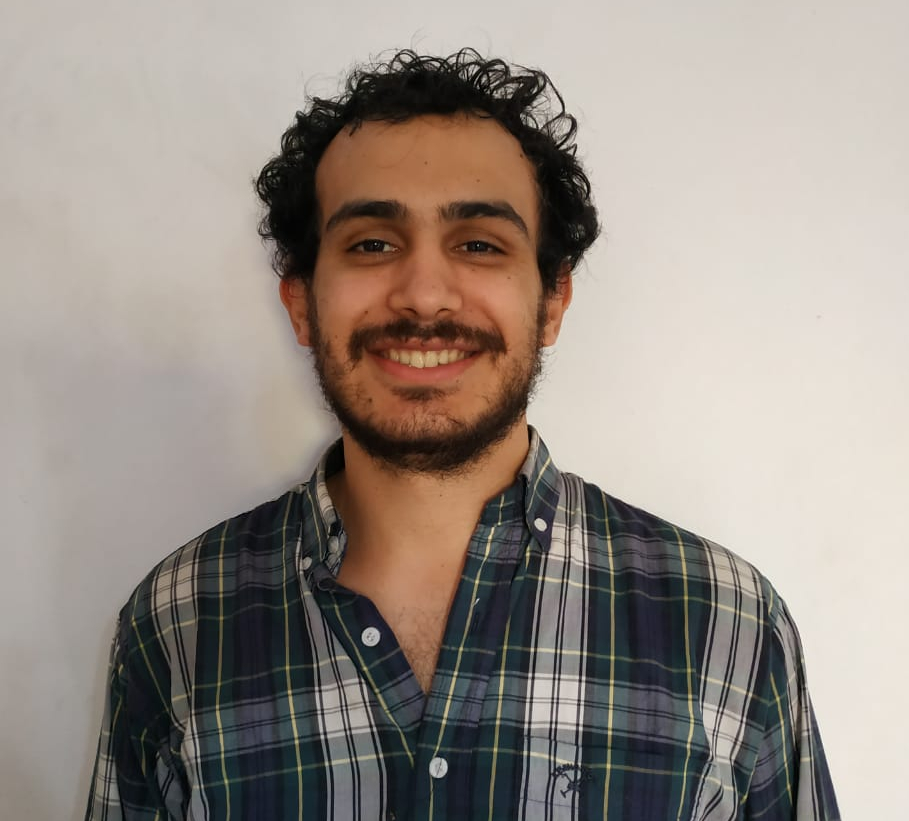
\includegraphics[width=0.25\textwidth]{pic4.jpeg}
\end{wrapfigure}

\MyName{Amadio, Camilo Leonel}
\MySlogan{Curriculum Vit\ae\ (\today)}

\sepspace
\sepspace
\sepspace
%%% Personal details
%%% ------------------------------------------------------------
\NewPart{}{}

\PersonalEntry{Dirección :}{Calle 12 N° 706 departamento 8A, La Plata, Argentina.}
\PersonalEntry{Teléfono :}{+ 54 221 155945496}
\PersonalEntry{Email:}{\href{mailto:camiloamadio57@gmail.com}{camiloamadio57@gmail.com}}
\PersonalEntry{Nacionalidad:}{Argentino.}
\PersonalEntry{Fecha de Nacimiento:}{27/04/1995}






%%% Work experience
%%% ------------------------------------------------------------
\NewPart{Educación}{}

\EducationEntry{Licenciatura en Física: } {2013-2019}{Facultad de Ciencias Exactas (FCE), \\ Universidad Nacional de La Plata (UNLP), La Plata, Argentina.}{

{\href{http://www.exactas.unlp.edu.ar/licenciatura_en_fisica}{Link}} pagina web de la licenciatura .
\begin{itemize}
\item{Fecha de graduación estimada: Mayo 2019. }
\item{Promedio Académico: 9.21 \\ {\href{https://drive.google.com/drive/folders/1je8C0gsbGixCF5rJo3fzQaqo1cs2mjX7?usp=sharing}{Link}} al Certificado Analítico.}
\item{Tesis de Licenciatura: Singularidades en Teorías Cuánticas de Campos.}
\end{itemize}

}
\sepspace

\EducationEntry{Workshop en Técnicas de Programación Científica:
}{2018}{Universidad Nacional de Quilmes, Quilmes, Argentina.}{\\
{\href{https://wtpc.github.io/}{Link}} a la pagina web del curso.\\
Curso presencial de 80 hs.\\
Temas Destacados:



\begin{itemize}
	\item{Gestión de código fuente (GIT).}
	\item{Lenguajes Compilados (C / FORTRAN).}
	\item{Debugging Y Profiling.}
	\item{Documentación Automática (Pydoc,Doxygen,Sphinx).}
	\item{Computación de alto rendimiento.}
	\end{itemize}}
\sepspace

\EducationEntry{Machine Learning, Data Science and Deep Learning with Python:
}{2018}{}{
12 hours {\href{https://www.udemy.com/data-science-and-machine-learning-with-python-hands-on/}{Curso de Udemy}}.
Temas Destacados:

\begin{itemize}
\item{Técnicas de Machine Learning: K-Means, Decision Trees, KNN, etc. }
\item{Redes Neuronales y Aprendizaje Profundo: Tensorflow, Keras.}
\end{itemize}
}


\sepspace

\NewPart{Becas}{}

\EducationEntry{Escuela de Verano:}
{2019}
{Instituto Balseiro, Centro Atómico de Bariloche, Bariloche, Argentina.}{\\
{\href{http://www.ib.edu.ar/component/k2/item/452-becas-de-verano.html}{Link}} a la beca.
\\ Beca de 160 horas desde 04/03/19 hasta 1/04/19. \\ 
Project: Sistema de control de posición para un adquisidor de imágenes de rayos x de alta resolución espacial, en el Laboratorio de Bajas Temperaturas.\\
{\href{https://drive.google.com/drive/folders/1y01BjDnIPS2QOX3Vo68r9A8HA9tstj1S}{Link}} al proyecto presentado.
}

\sepspace

\EducationEntry{Estimulo a las Vocaciones Científicas:}
{2018-2019}
{Instituto de Física de La Plata, La Plata, Buenos Aires, Argentina.}
{\\
{\href{http://evc.cin.edu.ar/}{Link}} a la beca.
\\ Beca de 12 horas semanales desde 04/03/19 hasta 29/04/19, proporcionada por el Consejo Interuniversitario Nacional. \\ 
Projecto: Funciones Espectrales en Teorías Cuánticas de Campos con Singularidades.
}


%%% Work experience
%%% ------------------------------------------------------------
\NewPart{Experiencia Laboral}{}

\sepspace



\WorkEntry{Ayudante Alumno Rentado:}
{}{2018-2019}
{Facultad de Ingeniería (FI), Universidad Nacional de La Plata (UNLP), La Plata, Argentina.}
{

Ayudante Alumno en {\href{https://www.ing.unlp.edu.ar/catedras/F0304/}{Matemática C}}, curso de segundo año.

Desde 14/03/18 hasta 31/03/19.

{\href{https://drive.google.com/drive/folders/1v960J-ofrC-xrrzCB4wOwtd4gdpVOSZy?usp=sharing}{Link} a la designación.}
}

\sepspace

\WorkEntry{Ayudante Alumno Rentado:}
{}{2018-2019}
{Facultad de Ingeniería (FI), Universidad Nacional de La Plata (UNLP), La Plata, Argentina.}
{

Ayudante Alumno en {\href{https://www.ing.unlp.edu.ar/catedras/F0305/}{Física II  }}, curso de segundo año.

Desde 14/03/18 hasta 31/03/19.

\href{https://drive.google.com/drive/folders/1vABkaZMn7Y_dWg1AbqDlz4lgAiekRv09?usp=sharing}{Link} a la designación.
}

\sepspace



\NewPart{Congresos}{}

\sepspace

\WorkEntry{103°  Reunión Nacional de la Asociación de Física Argentina:}{}{2018}{Ciudad de Buenos Aires, Argentina:}{

Congreso del 17/9/2018 al 21/9/2018.

Participante y expositor de póster.

{\href{https://drive.google.com/drive/folders/1WnbBy38R2___5leniTvo4lFK3aMaCwk7?usp=sharing}{Link}} a los certificados.
}


\newpage

\WorkEntry{102°  Reunión Nacional de la Asociación de Física Argentina:}{}{2018}{Ciudad de Buenos Aires, Argentina:}{}{2017}{La Plata,  Buenos Aires, Argentina}{

Congress from 26/9 to 29/9.

Participante y colaborador.

{\href{https://drive.google.com/drive/folders/166mUi8z6QCz5kGK86sLKj27jQiXhEmrc?usp=sharing}{Link}} al certificado.
}


%%% OTHER QUALIFICATIONS
%%% ------------------------------------------------------------
\NewPart{Cualificaciones}{}



\sepspace

\WorkEntry{Física:}{}{}{}{
\begin{itemize}
\item \textbf{Teoría Cuántica de Campos:} Tesis de licenciatura.
\item \textbf{Modelado de sistemas y simulaciones.}
\item \textbf{Técnicas Experimentales:} Reflectometría de Rayos x, Sputtering, Espectrofotómetro óptico, \\ Espectrofotómetro de transformada de fourier, Osciloscopio.
\end{itemize}
}

\sepspace

\WorkEntry{Matemática:}{}{}{}{
\begin{itemize}
\item \textbf{Álgebra Lineal.}
\item \textbf{Análisis Matemático.}
\item \textbf{Ecuaciones Diferenciales.}
\item \textbf{Análisis de Variable Compleja.} 
\end{itemize}
}

\sepspace

\WorkEntry{Programación:}{}{}{}{
\begin{itemize}
\item \textbf{Python:} Programación orientada a objetos, Simulaciones, Análisis de Datos, Machine Learning (TensorFlow/Keras).
\item \textbf{Fortran 90:} Simulaciones.
\item \textbf{Arduino:} Arduino Uno. {\href{https://drive.google.com/drive/folders/1y01BjDnIPS2QOX3Vo68r9A8HA9tstj1S}{Link }} al projecto en el Instituto Balseiro.
\item \textbf{Wolfram Mathematica.} 
\item \textbf{LaTeX.}
\end{itemize}
}

\sepspace

\WorkEntry{Habilidades Computacionales:}{}{}{}{
\begin{itemize}
\item \textbf{Usuario Linux.}
\item \textbf{Usuario Windows.}
\item \textbf{Microsoft Office.}
\end{itemize}
}

\sepspace

%%% LANGUAGES
%%% ------------------------------------------------------------
\NewPart{IDIOMAS}{}

\begin{itemize}
\item \textbf{Español:} Lengua Materna.
\item \textbf{Inglés:} Fluido.
\item \textbf{Hebreo:} Actualmente estudiando en {\href{https://rosenhebrewschool.com/}{Rosen School of Hebrew}}.
\end{itemize}


\begin{comment}


%%% LANGUAGES
%%% ------------------------------------------------------------
\NewPart{Interests and personality}{}

\Text{Sports and outdoor activities, mainly freeride skiing. The last couple of years I have been competing in freeride skiing and been partially living in the Swiss Alps. Through my skiing I have also developed my ski production. My friends and family form my other big interest. I see myself as a happy, outgoing and reliable person. I am a problem solver and no challenge is too big. The result of my work is often better than expected.}




\NewPart{Expected Salary:}{}

\WorkEntry{}{}{}{}{
\begin{itemize}
\item{My expected salary is in the 700 to 800 USD range.}
\end{itemize}
}

\end{comment}


\end{document}
